\bigskip
\begin{center}
\textbf{\Large \color{red}This tutorial is currently under construction/revision.}
\end{center}
\bigskip

\section{Overview}


This tutorial demonstrates how to accommodate variation in the substitution process across sites of an alignment.
In the preceding tutorials, we assumed that all sites in an alignment evolved under an identical substitution process.
This assumption is likely to be violated in real datasets.  
Here, we will demonstrate how to specify---and select among---alternative \emph{mixed models} using \RevBayes.
This is commonly referred to as partitioned-data analysis, where two or more subsets of sites in our alignment are assumed to evolve under distinct processes.
% and different partition configurations of aligned DNA sequences. 

\subsection{Requirements}
We assume that you have previously completed the following tutorials:
\begin{itemize}
\item RB\_Getting\_Started
\item RB\_Data\_Tutorial
\item RB\_CTMC\_Tutorial
\item RB\_BayesFactor\_Tutorial
\end{itemize}
Accordingly, we will assume that you know how to execute and load data into \RevBayes, are familiar with some basic commands, and know how to perform Bayes factor comparisons to select among competing substitution models.



%%%%%%%%
%%   Data   %%
%%%%%%%%
\section{Data and files}

We provide several data files that we will use in this tutorial; these are the same datasets that we have used in previous tutorials.
In the \cl{data} folder, you will find the following files
\begin{itemize}
\item
\cl{primates\_cytb.nex}: Alignment of the \textit{cytochrome b} subunit from 23 primates representing 14 of the 16 families (\textit{Indriidae} and \textit{Callitrichidae} are missing).
\item
\cl{primates\_16s.nex}: Alignment of the \textit{16s ribosomal RNA} gene from the same 23 primates species.
\item
\cl{primates\_cox2.nex}: Alignment of the \textit{COX-2} gene from the same 23 primates species.
\end{itemize}



\section{Introduction}

Variation in the evolutionary process across the sites of nucleotide sequence alignments is well established, and is an increasingly pervasive feature of datasets composed of gene regions sampled from multiple loci and/or different genomes.
Inference of phylogeny from these data demands that we adequately model the underlying process heterogeneity; failure to do so can lead to biased estimates of phylogeny and other parameters \citep{Brown2007}.
%To accommodate process heterogeneity within and/or between various gene(omic) regions, we will evaluate the support for various partition schemes using Bayes factors to compare the marginal likelihoods of the candidate partition schemes.

Accounting for process heterogeneity involves adopting a `mixed-model' approach, \citep{Ronquist2003} in which the sequence alignment is first parsed into a number of partitions that are intended to capture plausible process heterogeneity within the data.
The determination of the partitioning scheme is guided by biological considerations regarding the dataset at hand.
For example, we might wish to evaluate possible variation in the evolutionary process within a single gene region (\EG between stem and loop regions of ribosomal sequences), or among gene regions in a concatenated alignment (\EG comprising multiple nuclear loci and/or gene regions sampled from different genomes).
The choice of partitioning scheme is up to the investigator and many possible partitions might be considered for a typical dataset.

%Next, a substitution model is specified for each predefined process partition (using a given model-selection criterion, such as Bayes factors).
In this exercise, we assume that each partition evolved under an independent general-time reversible model with gamma-distributed rates across sites (GTR+$\Gamma$). 
Under this model the observed data are conditionally dependent on the exchangeability rates ($\theta$), stationary base frequencies ($\pi$), and the degree of gamma-distributed among-site rate variation ($\alpha$), as well as the unrooted tree topology ($\Psi$) and branch lengths ($\nu$).
We show the graphical model representation of the GTR+$\Gamma$ mode in Figure \ref{gtrgmfig}. 
When we assume different GTR+$\Gamma$ models for each partitions, this results in a composite model, in which all sites are assumed to share a common, unrooted tree topology and proportional branch lengths, but subsets of sites (`data partitions') are assumed to have independent substitution model parameters.
This composite model is referred to as a \emph{mixed model}. 
%\taha{need to change the graphical model above to have the same symbols as in this paragraph since this refers to the figure \ref{pipeline} and it may be harder to change that figure.}



Finally, we perform a separate MCMC simulation to approximate the joint posterior probability density of the phylogeny and other parameters.  Note that, in this approach, the mixed model is a fixed assumption of the inference (\IE the parameter estimates are conditioned on the specified mixed model), and the parameters for each process partition are independently estimated.

For most sequence alignments, several (possibly many) partition schemes of varying complexity are plausible {\it a priori}, which therefore requires a way to objectively identify the partition scheme that balances estimation bias and error variance associated with under- and over-parameterized mixed models, respectively.
Increasingly, mixed-model selection is based on \textit{Bayes factors} \citep[{\it e.g.},][]{suchard01}, which involves first calculating the marginal likelihood under each candidate partition scheme and then comparing the ratio of the marginal likelihoods for the set of candidate partition schemes \citep{brandley05,nylander04,mcguire07}.
The analysis pipeline that we will use in this tutorial is depicted in Figure \ref{pipeline}.
\begin{figure}[h!]
\centering
\fbox{\includegraphics[width=6.8in,angle=0]{\ResourcePath figures/pipeline.eps}}
\caption{\small The analysis pipeline for Exercise 1. We will explore three partition schemes for the conifer dataset.
The first model (the `uniform model', $M_0$) assumes that all sites evolved under a common GTR+$\Gamma$ substitution model.
The second model (the `moderately partitioned' model, $M_1$) invokes two data partitions corresponding to the two gene regions (atpB and rbcL), and assumes each subset of sites evolved under an independent GTR+$\Gamma$ model.
The final mixed model (the `highly partitioned' model, $M_2$) invokes four data partitions---the first partition corresponds to the atpB gene region, and the remaining partitions correspond to the three codon positons of the rbcL gene region---and each data partition is assumed evolved under an independent GTR+$\Gamma$ substitution model.
Note that we assume that all sites share a common tree topology, $\Psi$, and branch-length proportions, $\nu$, for each of the candidate partition schemes.
We perform two separate sets of analyses for each mixed model---a Metropolis-coupled MCMC simulation to approximate the joint posterior probability density of the mixed-model parameters, and a `stepping-stone' MCMC simulation to approximate the marginal likelihood for each mixed model.
The resulting marginal-likelihood estimates are then evaluated using Bayes factors to assess the fit of the data to the three candidate mixed models.  
}
\label{pipeline}
\end{figure}
 
\bigskip
\section{Two-gene analysis}\label{secUnif} 

The first section of this exercise involves 
(1) setting up a uniform GTR+$\Gamma$ model for an alignment comprising two genes, 
(2) approximating the posterior probability of the tree topology and branch lengths (and all other parameters) using MCMC,  
(3) summarizing the MCMC output by computing the maximum a posteriori tree. 

All of the files for this analysis are provided for you and you can run these without significant effort using the \cl{source()} function in the \RevBayes~console:
{\tt \begin{snugshade*}
\begin{lstlisting}
source("RevBayes_scripts/uniform.Rev")
\end{lstlisting}
\end{snugshade*}}

If everything loaded properly, then you should see the program begin running the Markov chain Monte Carlo analysis needed for estimating the posterior distribution. If you continue to let this run, then you will see it output the states of the Markov chain once the MCMC analysis begins. (It is worth noting, however, that the file \cl{quick\_uniform.Rev} performs shorter runs with fewer generations for a faster run time.)

\bigskip
\subsection{Full Model Specification}

\subsubsection{Load Data}

First load in the sequences using the \cl{readDiscreteCharacterData()} function. 
{\tt \begin{snugshade*}
\begin{lstlisting}
data_16s <- readDiscreteCharacterData("data/primates_16s_rrna.nex")
data_cytb <- readDiscreteCharacterData("data/primates_cytb.nex")
\end{lstlisting}
\end{snugshade*}}
Executing these lines initializes each data matrix as their respective \Rev~variables. 
Since the first step in this exercise is to assume a single model for both genes, we need to combine the two datasets.
Concatenate the two data matrices using the \cl{concatenate()} function. This returns a single data matrix with both genes.

{\tt \begin{snugshade*}
\begin{lstlisting}
data <- concatenate(data_16s, data_cytb)
\end{lstlisting}
\end{snugshade*}}

To report the current value of any variable, simply type the variable name and press enter. For the \cl{data} matrix, this provides information about the alignment:


{\tt \begin{snugshade*}
\begin{lstlisting}

   DNA character matrix with 23 taxa and 2782 characters
   =====================================================
   Origination:                   primates_16s_rrna.nex
   Number of taxa:                23
   Number of included taxa:       23
   Number of characters:          2782
   Number of included characters: 2782
   Datatype:                      DNA

\end{lstlisting}
\end{snugshade*}}


Next we will specify some useful variables based on our dataset. The variable \cl{data} has \textit{member functions} that we can use to retrieve information about the dataset. 
These include the number of species (\cl{n\_species}), the tip labels (\cl{names}), and the number of internal branches (\cl{n\_branches}).
Each of these variables will be necessary for setting up different parts of our model.
{\tt \begin{snugshade*}
\begin{lstlisting}
names <- data.names()
n_species <- data.ntaxa()
n_branches <- 2 * n_species - 3 
\end{lstlisting}
\end{snugshade*}}

Now we can proceed with building our GTR$+\Gamma$ model.

\textbf{\textit{The GTR Parameters}}

The first step in this exercise involves estimating the marginal likelihood of our model assuming an unpartitioned alignment. 
This corresponds to the assumption that the process that gave rise to our data was homogeneous across all sites. 
Specifically, we will assume that both genes evolved under the same GTR$+\Gamma$ model (Fig.~\ref{pipeline}). 

First, we will define and specify a prior on the exchangeability rates of the GTR model. We will use a flat Dirichlet prior distribution on these six rates. To do this, we must begin by defining a constant node that specifies the vector of concentration values of the Dirichlet prior using the \cl{v()} function:
{\tt \begin{snugshade*}
\begin{lstlisting}
er_prior <- v(1,1,1,1,1,1) 
\end{lstlisting}
\end{snugshade*}}


The constant node \cl{er\_prior} corresponds to the node labeled $e$ in the graphical model depicted in Figure \ref{gtrgmfig}. 
The vector function, \cl{v()}, creates a vector of six values. 
Display the current value of \cl{er\_prior} by simply typing the variable name:
{\tt \begin{snugshade*}
\begin{lstlisting}
er_prior
|*       [ 1, 1, 1, 1, 1, 1 ]
\end{lstlisting}
\end{snugshade*}}
This node defines the parameters of the Dirichlet prior distribution on the exchangeability rates. Thus, we can create a stochastic node for the exchangeability rates using the \cl{dnDirichlet()} function, which takes a vector of values as an argument and the \cl{\rbdn} operator. Together, these create a stochastic node named \cl{er} ($\theta$ in Figure \ref{gtrgmfig}): 
{\tt \begin{snugshade*}
\begin{lstlisting}
er ~ dnDirichlet(er_prior)
\end{lstlisting}
\end{snugshade*}}


The Dirichlet distribution assigns probability densities to grouped parameters: {\it e.g.}, those that measure proportions and must sum to 1. 
Above, we specified a 6-parameter Dirichlet prior on the relative rates of the GTR model, where the placement of each value specified represents one of the 6 relative rates: (1) $A\leftrightarrows C$, (2) $A\leftrightarrows G$, (3) $A\leftrightarrows T$, (4) $C\leftrightarrows G$, (5) $C\leftrightarrows T$, (6) $G\leftrightarrows T$. 
The input parameters of a Dirichlet distribution are called shape parameters or concentration parameters and a value is specified for each of the 6 GTR rates. 
The expectation and variance for each variable are related to the sum of the shape parameters.
The prior above is a `flat' or symmetric Dirichlet since all of the shape parameters are equal (1,1,1,1,1,1), thus we are specifying a model that allows for equal rates of change between nucleotides, such that the expected rate for each is equal to $\frac{1}{6}$ \citep{zwickl04}.
Figure \ref{dirichletFig}a shows the probability density of each rate under this model.
If we parameterized the Dirichlet distribution such that all of the parameters were equal to 100, this would also specify a prior with an expectation of equal exchangeability rates (Figure \ref{dirichletFig}b). 
However, by increasing the shape parameters of the Dirichlet distribution, \cl{er\_prior <- v(100,100,100,100,100,100)}, would heavily restrict the MCMC from sampling sets of GTR rates in which the values were not equal or very nearly equal ({\it i.e.}, this is a very {\em informative} prior). 
We can consider a different Dirichlet parameterization if we had strong prior belief that transitions and transversions occurred at different rates.
In this case, we could specify a more informative prior density: \cl{er\_prior <- v(4,8,4,4,8,4)}. 
Under this model, the expected rate for transversions would be $\frac{4}{32}$ and the expected rate for transitions would equal $\frac{8}{32}$, and there would be greater prior probability on sets of GTR rates that matched this configuration (Figure \ref{dirichletFig}c). 
An alternative informative prior would be one where we assumed that each of the 6 GTR rates had a different value conforming to a Dirichlet(2,4,6,8,10,12). 
This would lead to a different prior probability density for each rate parameter (Figure \ref{dirichletFig}d).
Without strong prior knowledge about the pattern of relative rates, however, we can better capture our statistical uncertainty with a vague prior on the GTR rates. 
Notably, all patterns of relative rates have the same probability density under \cl{er\_prior <- v(1,1,1,1,1,1)}.
\begin{figure}[h!]
\centering
\fbox{\includegraphics[width=5in,angle=-90]{\ResourcePath figures/dirichlet_rates.eps}}
\caption{\small Four different examples of Dirichlet priors on exchangeability rates.}
\label{dirichletFig}
\end{figure}

For each stochastic node in our model, we must also specify a proposal mechanism if we wish to sample that value. 
The Dirichlet prior on our parameter \cl{er} creates a \href{http://en.wikipedia.org/wiki/Simplex}{\textit{simplex}} of values that sum to 1. 
In RevBayes, there are many different proposal mechanisms -- called \textit{moves} -- and each move operates on a specific data type (called RevType). 
Check the RevType of the variable \cl{er} using the \cl{structure()} function:
{\tt \small \begin{snugshade*}
\begin{lstlisting}
structure(er)

|*  _variable     = er <0x7ffed8449370>
|*  _RevType      = Simplex
|*  _RevTypeSpec  = [ Simplex, RealPos[], ModelContainer, Container, RevObject ]
|*  _value        = [ 0.00308506, 0.491487, 0.186317, 0.0275106, 0.1982...
|*  _size         = 6
|*  _dagNode      = er <0x7ffed8448bb0>
|*  _dagType      = Stochastic DAG node
|*  _refCount     = 1
|*  _distribution = <0x7ffed8448cf0>
|*  _touched      = TRUE
|*  _clamped      = FALSE
|*  _lnProb       = -inf
|*  _storedLnProb = 6.95325e-310
|*  _parents      = [ er_prior <0x7ffed8449250> ]
|*  _children     = [  ]
\end{lstlisting}
\end{snugshade*}}

The \cl{structure()} function -- which has an accepted abbreviation of \cl{str()} -- is verbose and provides a lot of information that may at first appear confusing. 
In particular, this function provides the \href{http://en.wikipedia.org/wiki/Memory_address}{\textit{memory addresses}} of the node, its parent node(s), and the distribution. 
These strings indicate the location of the variable in computer memory. 
Thus, if you view the structure of your \cl{er} node, these sequences of numbers will be different from the ones in the box above. 
Much of this information is helpful primarily for troubleshooting and debugging purposes, however, the components that you may want to look at are: \cl{RevType}, \cl{value}, \cl{dagType}, \cl{clamped}, \cl{lnProb}, and the names of the \cl{variable}, \cl{parents}, and \cl{children}.

We must create a vector containing all of the moves for each of our stochastic nodes. 
This vector will be passed in to the function constructing our MCMC or power posterior runs.
All moves in the Rev language are called \cl{mv*}, where \cl{*} is a wild card for the move name. 
Initialize the first element of our vector of moves by setting the proposal on the exchangeability rates:

{\tt\small \begin{snugshade*}
\begin{lstlisting}
moves[++mi] = mvSimplexElementScale(er, alpha=10, tune=true, weight=3) 
\end{lstlisting}
\end{snugshade*}}


The various proposal mechanisms available in \RevBayes~each require specific input arguments. 
The \cl{mvSimplexElementScale} move can only operate on a simplex and the first argument is the stochastic node that you wish to update. 
The variable node is followed by three more arguments: (1) \cl{alpha} is the \textit{tuning parameter} of the move and controls the size of the proposal; (2) by setting \cl{tune=true} we are telling the program to adjust the tuning parameter if the acceptance rate of the proposal is too high or too low -- the target for this move is an acceptance rate of 0.44; (3) the \cl{weight} specifies how frequently this move is performed at each step in the Markov chain. 

It is important to note that by default, a single generation in RevBayes updates all stochastic nodes in proportion to the \cl{weight} argument specified. 
This approach is different from many phylogenetic MCMC programs -- such as MrBayes -- which only perform one move per MCMC iteration. 
Instead, for each generation in RevBayes, a \textit{move list} is carried out in random order. 
By setting \cl{weight=3} above, we are ensuring that the new values are proposed for \cl{er} three times per iteration. 
Thus, if you set \cl{weight=0.5} the move will only have a 50\% chance of occurring at each generation. 
Essentially, the \cl{weight} argument for each move indicates the number of times it will be performed.
If you keep all of the move weights set to the values specified in this tutorial for the uniform model, you will have set 20 different moves and the MCMC simulator will execute 38 moves per generation.
This is a practical approach for MCMC analysis using complex models and is used by several other programs (\href{http://megasun.bch.umontreal.ca/People/lartillot/www/index.htm}{Phylobayes}, \href{http://hydrodictyon.eeb.uconn.edu/projects/phycas/index.php/Phycas_Home}{Phycas}, \href{http://www.bali-phy.org/}{Bali-Phy}).
However, because RevBayes is updating many parameters each generation, it is not straightforward to compare run-times with a program like MrBayes that only performs approximately one update per generation. 
Furthermore, using this approach to MCMC simulation, you can sufficiently sample the chain in fewer generations while sampling more frequently than you would in programs that only perform one update per step.

We can use the same type of distribution as a prior on the 4 stationary frequencies ($\pi_A, \pi_C, \pi_G, \pi_T$) since these parameters also represent proportions. 
Specify a flat Dirichlet prior density on the base frequencies:
{\tt \begin{snugshade*}
\begin{lstlisting}
sf_prior <- v(1,1,1,1) 
sf ~ dnDirichlet(sf_prior)
\end{lstlisting}
\end{snugshade*}}

The node \cl{sf} represents the $\pi$ node in Figure \ref{gtrgmfig}.
Now add the simplex scale move on the stationary frequencies to the moves vector:
{\tt \small \begin{snugshade*}
\begin{lstlisting}
moves[2] <- mvSimplexElementScale(sf, alpha=10, tune=true, weight=2)  
\end{lstlisting}
\end{snugshade*}}

We can finish setting up this part of the model by creating a deterministic node for the GTR rate matrix \cl{Q}. 
The \cl{fnGTR()} function takes a set of exchangeability rates and a set of base frequencies to compute the rate matrix used when calculating the likelihood of our model.
{\tt \begin{snugshade*}
\begin{lstlisting}
Q := fnGTR(er,sf)
\end{lstlisting}
\end{snugshade*}}


\textbf{\textit{Gamma-Distributed Site Rates}}


We will also assume that the substitution rates vary among sites according to a gamma distribution, which has two parameters: the shape parameter, $\alpha$, and the rate parameter, $\beta$. 
In order that we can interpret the branch lengths as the expected number of substitutions per site, this model assumes that the mean site rate is equal to 1.
%Consequently, we wish to specify a gamma distribution with a mean of 1.
The mean of the gamma is equal to $\alpha/\beta$, so a mean-one gamma is specified by setting the two parameters to be equal, $\alpha=\beta$.
Therefore, we need only consider the single shape parameter, $\alpha$ \citep{yang94a}. 
The degree of among-site substitution rate variation (ASRV) is inversely proportional to the value of the shape parameter---as the value of $\alpha$-shape parameter increases, the gamma distribution increasingly resembles a normal distribution with decreasing variance, which corresponds to decreasing levels of ASRV (Figure \ref{asrhGammaFig}).
If $\alpha = 1$, then the gamma distribution collapses to an exponential distribution with a rate parameter equal to $\beta$.
By contrast, when the value of the $\alpha$-shape parameter is $< 1$, the gamma distribution assumes a concave distribution that places most of the prior density on low rates but allows some prior mass on sites with very high rates, which corresponds to high levels of ASRV (Figure \ref{asrhGammaFig}).

\begin{figure}[h]
\centering
\fbox{\includegraphics[width=2.5in,angle=-90]{\ResourcePath figures/asrh_gamma.eps}}
\caption{\small The probability density of mean-one gamma-distributed rates under different shape parameters.}
\label{asrhGammaFig}
\end{figure}


Alternatively, we might not have good prior knowledge about the variance in site rates, thus we can place an uninformative, or diffuse prior on the shape parameter.
For this analysis, we will use an exponential distribution with a rate parameter, \cl{shape\_prior}, equal to \cl{0.05}.
Under an exponential prior, we are placing non-zero probability on values of $\alpha$ ranging from 0 to $\infty$. 
The rate parameter, often denoted $\lambda$, of an exponential distribution controls both the mean and variance of this prior such that the expected (or mean) value of $\alpha$ is:
$\mathbb{E}[\alpha] = \frac{1}{\lambda}.$
Thus, if we set $\lambda=0.05$, then $\mathbb{E}[\alpha] = 20$.

Create a constant node called \cl{shape\_prior} for the rate parameter of the exponential prior on the gamma-shape parameter
{\tt\begin{snugshade*}
\begin{lstlisting}
shape_prior <- 0.05                                                                             
\end{lstlisting}
\end{snugshade*}}

Then create a stochastic node called \cl{shape} to represent the $\alpha$ node in Figure \ref{gtrgmfig}, with an exponential density as a prior:
{\tt\begin{snugshade*}
\begin{lstlisting}
shape ~ dnExponential(shape_prior)

\end{lstlisting}
\end{snugshade*}}

The way the ASRV model is implemented involves discretizing the mean-one gamma distribution into a set number of rate categories. Thus, we can analytically marginalize over the uncertainty in the rate at each site. To do this, we need a deterministic node that is a vector of rates calculated from the gamma distribution and the number of rate categories. The \cl{fnDiscretizeGamma()} function returns this deterministic node and takes three arguments: the shape and rate of the gamma distribution and the number of categories. Since we want to discretize a mean-one gamma distribution, we can pass in \cl{shape} for both the shape and rate.

Initialize the \cl{gamma\_rates} deterministic node vector using the  \cl{fnDiscretizeGamma()} function with \cl{4} bins:
{\tt \begin{snugshade*}
\begin{lstlisting}
gamma_rates := fnDiscretizeGamma( shape, shape, 4 )
\end{lstlisting}
\end{snugshade*}}



The random variable that controls the rate variation is the stochastic node \cl{shape}. This variable is a single, real positive value (\cl{RevType = RealPos}). 
We will apply a simple scale move to this parameter.
The scale move's tuning parameter is called \cl{lambda} and this value dictates the size of the proposal.
{\tt \begin{snugshade*}
\begin{lstlisting}
moves[3] <- mvScale(shape, lambda=1.0, tune=true, weight=2.0)\end{lstlisting}
\end{snugshade*}}


\textbf{\textit{Tree Topology and Branch Lengths}}

The tree topology and branch lengths are also stochastic nodes in our model. 
In Figure \ref{gtrgmfig}, the tree topology is denoted $\Psi$ and the length of the branch leading to node $i$ is $\nu_i$.

We will assume that all possible labeled, unrooted tree topologies have equal probability. This is the \cl{dnUniformTopology()} distribution in RevBayes. Specify the \cl{topology} stochastic node by passing in the number of species \cl{n\_species} and tip labels \cl{names} to the \cl{dnUniformTopology()} distribution:
{\tt \begin{snugshade*}
\begin{lstlisting}
topology ~ dnUniformTopology(n_species, names)
\end{lstlisting}
\end{snugshade*}}

For some types of stochastic nodes there are several available moves. 
Often the different moves explore parameter space in a different way and nothing prevents one from using multiple different moves to improve mixing. 
For the unrooted tree topology, we can use both a nearest-neighbor interchange move (\cl{mvNNI}) and a subtree-prune and regrafting move (\cl{mvSPR}). These moves do not have tuning parameters associated with them, thus you only need to pass in the \cl{topology} node and \cl{weight} 
{\tt \begin{snugshade*}
\begin{lstlisting}
moves[4] <- mvNNI(topology, weight=10.0)
moves[5] <- mvSPR(topology, weight=5.0)
\end{lstlisting}
\end{snugshade*}}


Next we have to create a stochastic node for each of the $2N-3$ branches in our tree (where $N=$ \cl{n\_species}). 
We can do this using a \cl{for} loop --- this is a plate in our graphical model. In this loop, we can create each branch-length node and assign each move. Copy this entire block of Rev code into the console:
{\tt \small \begin{snugshade*}
\begin{lstlisting}
mi <- 5
for (i in 1:n_branches) {
   br_lens[i] ~ dnExponential(10.0)
   moves[mi++] <- mvScale(br_lens[i],lambda=1,tune=true,weight=1) 
}
\end{lstlisting}
\end{snugshade*}}

It is convenient to monitor a deterministic variable of the branch lengths. In MrBayes, \textit{tree length} was reported to the log file instead of the length of each branch. The tree length is the sum of all branch lengths and this can be computed using the \cl{sum()} function which calculates the sum of any vector of values.
{\tt \begin{snugshade*}
\begin{lstlisting}
tree_length := sum(br_lens)
\end{lstlisting}
\end{snugshade*}}

Finally, we can create a branch-length phylogeny by combining the tree topology and branch lengths using the \cl{treeAssembly()} function, which applies the value of the $i^{th}$ member of the \cl{br\_lens} vector to the branch leading to the $i^{th}$ node in \cl{topology}. Thus, the \cl{phylogeny} variable is a deterministic node: 

{\tt \begin{snugshade*}
\begin{lstlisting}
phylogeny := treeAssembly(topology, br_lens)
\end{lstlisting}
\end{snugshade*}}



\textbf{\textit{Putting it All Together}}

Now that we have initialized virtually all of our model parameters and we can link all of the parts in the stochastic node that will be clamped by the data. 
The sequence substitution model is a distribution called the \textit{phylogenetic continuous-time Markov chain} and we use the \cl{dnPhyloCTMC} constructor function to create this node.
This distribution requires several input arguments: (1) the \cl{tree} with branch lengths, (2) the instantaneous rate matrix \cl{Q}, the node characterizing the rate variation across sites (though \cl{siteRates} can be omitted if you do not assume rate variation across sites), (3) \cl{nSites} is the number of sites in the alignment, and (4) the \cl{type} of character data.
{\tt \begin{snugshade*}
\begin{lstlisting}
phyloSeq ~ dnPhyloCTMC(tree=phylogeny, Q=Q, siteRates=gamma_rates, nSites=data.nchar(1), type="DNA")
\end{lstlisting}
\end{snugshade*}}


Once the character evolution model has been created, we can attach our sequence data to the tip nodes in the tree.
{\tt \begin{snugshade*}
\begin{lstlisting}
phyloSeq.clamp(data)
\end{lstlisting}
\end{snugshade*}}
When this function is called, \RevBayes~sets each of the stochastic nodes representing the tip nodes of the tree to the sequence corresponding to that species in the alignment. 
This essentially tells the program that this is where the DAG ends and the states of the tip nodes are fixed. 

Now we can wrap up the whole model to conveniently access the DAG. To do this, we only need to give the \cl{model()} function a single node. With this node, the \cl{model()} function can find all of the other nodes by following the arrows in the graphical model:
{\tt \begin{snugshade*}
\begin{lstlisting}
mymodel = model(Q)
\end{lstlisting}
\end{snugshade*}}

Now we have specified a simple, single-partition analysis---each parameter of the model will be estimated from every site in our alignment.
If we inspect the contents of \cl{mymodel} we can review all of the nodes in the DAG:
{\tt \begin{snugshade*}
\begin{lstlisting}
mymodel
\end{lstlisting}
\end{snugshade*}}

\bigskip
{\large \textcolor{mycol}{\textsc{Perform MCMC Analysis Under the Uniform Model}}}

This section will cover setting up the MCMC sampler and summarizing the posterior distribution of trees. 

\textbf{\textit{Specify Monitors}}

For our MCMC analysis we need to set up a vector of \textit{monitors} to save the states of our Markov chain. 
The monitor functions are all called \cl{mn*}, where \cl{*} is the wildcard representing the monitor type.
First, we will initialize the model monitor using the \cl{mnModel} function. This creates a new monitor variable that will output the states for all model parameters when passed into a MCMC function. 
{\tt \begin{snugshade*}
\begin{lstlisting}
monitors[1] = mnModel(filename="output/conifer_uniform.log", printgen=100)
\end{lstlisting}
\end{snugshade*}}

The \cl{mnFile} monitor will record the states for only the parameters passed in as arguments. We use this monitor to specify the output for our sampled trees and branch lengths.

{\tt \begin{snugshade*}
\begin{lstlisting}
monitors[2] = mnFile(filename="output/conifer_uniform.trees",printgen=100, phylogeny)
\end{lstlisting}
\end{snugshade*}}


Finally, create a screen monitor that will report the states of specified variables to the screen with \cl{mnScreen}:
{\tt \begin{snugshade*}
\begin{lstlisting}
monitors[3] = mnScreen(printgen=10, separator = " | ", tree_length)
\end{lstlisting}
\end{snugshade*}}

\textbf{\textit{Initialize and Run MCMC}}

With a fully specified model, a set of monitors, and a set of moves, we can now set up the MCMC algorithm that will sample parameter values in proportion to their posterior probability. The \cl{mcmc()} function will create our MCMC object:
{\tt \begin{snugshade*}
\begin{lstlisting}
mymcmc = mcmc(mymodel, monitors, moves)
\end{lstlisting}
\end{snugshade*}}


We can run the \cl{.burnin()} member function if we wish to pre-run the chain and discard the initial states. 
{\tt \begin{snugshade*}
\begin{lstlisting}
mymcmc.burnin(generations=10000,tuningInterval=1000)
\end{lstlisting}
\end{snugshade*}}


Now, run the MCMC:
{\tt \begin{snugshade*}
\begin{lstlisting}
mymcmc.run(generations=30000)
\end{lstlisting}
\end{snugshade*}}

When the analysis is complete, you will have the monitor files in your output directory.


\textbf{\textit{Summarize the MCMC Output}}

Methods for visualizing the marginal densities of parameter values are not currently available in \RevBayes. Thus, it is important to use programs like Tracer \citep{rambaut09} to evaluate mixing and non-convergence. (RevBayes does, however, have a tool for convergence assessment called \cl{beca}.)

\RevBayes~can also summarize the tree samples by reading in the tree-trace file:
{\tt \begin{snugshade*}
\begin{lstlisting}
treetrace = readTreeTrace("output/conifer_uniform.trees")
treetrace.summarize()
\end{lstlisting}
\end{snugshade*}}


The \cl{mapTree()} function will summarize the tree samples and write the maximum a posteriori tree to file:
{\tt \begin{snugshade*}
\begin{lstlisting}
mapTree(treetrace,"output/conifer_uniform_map.tre")
\end{lstlisting}
\end{snugshade*}}


\bigskip
\subsection{Partitioning by Gene Region}\label{secByGene}

The uniform model used in the previous section assumes that all sites in the alignment evolved under the same process described by a shared tree, branch length proportions, and parameters of the GTR+$\Gamma$ substitution model.
However, our alignment contains two distinct gene regions---atpB and rbcL---so we may wish to explore the possibility that the substitution process differs between these two gene regions.
This requires that we first specify the data partitions corresponding to these two genes, then define an independent substitution model for each data partition. 

\textbf{\textit{Clear Workspace and Reload Data}}

{\tt \begin{snugshade*}
\begin{lstlisting}
clear()
\end{lstlisting}
\end{snugshade*}}

Since we wish to avoid individually specifying each parameter of the GTR+$\Gamma$ model for each of our data partitions, we can \textit{loop} over our datasets and create vectors of nodes.
To do this, we begin by creating a vector of data file names:
{\tt \begin{snugshade*}
\begin{lstlisting}
filenames <- v("data/conifer_atpB.nex", "data/conifer_rbcL.nex")
\end{lstlisting}
\end{snugshade*}}

Set a variable for the number of partitions:
{\tt \begin{snugshade*}
\begin{lstlisting}
n_parts <- filenames.size()
\end{lstlisting}
\end{snugshade*}}

And create a vector of data matrices called \cl{data}:
{\tt \begin{snugshade*}
\begin{lstlisting}
for (i in 1:n_parts){
   data[i] <- readDiscreteCharacterData(filenames[i])[1]
}
\end{lstlisting}
\end{snugshade*}}

Next, we can initialize some important variables. This does require, however, that both of our alignments have the same number of species and matching tip names.
{\tt \begin{snugshade*}
\begin{lstlisting}
n_species <- data[1].ntaxa()
names <- data[1].names()
n_branches <- 2 * n_species - 3
\end{lstlisting}
\end{snugshade*}}


\subsection{Specify the Parameters by Looping Over Partitions}

We can avoid creating unique names for every node in our model if we use a \cl{for} loop to iterate over our partitions. Thus, we will only have to type in our entire GTR+$\Gamma$ model parameters once. 
This will produce a vector for each of the unlinked parameters --- e.g., there will be a vector of \cl{shape} nodes where the stochastic node for the first partition (atpB) will be \cl{shape[1]} and the stochastic node for the second partition (rbcL) will be called \cl{shape[2]}.
{\tt \small \begin{snugshade*}
\begin{lstlisting}
mi = 0 # an iterator for the move vector
for (i in 1:n_parts){
  ## index i=1 : atpB gene ##
  ## index i=2 : rbcL gene ##
  
  # Exchangeability rates #
  er_prior[i] <- v(1,1,1,1,1,1)
  er[i] ~ dnDirichlet(er_prior[i])
  moves[++mi] = mvSimplexElementScale(er[i], alpha=10, tune=true, weight=3) 

  # Stationary base frequencies #
  sf_prior[i] <- v(1,1,1,1)
  sf[i] ~ dnDirichlet(sf_prior[i])
  moves[++mi] = mvSimplexElementScale(sf[i], alpha=10, tune=true, weight=2) 

  # Instantaneous rate matrix (deterministic) #
  Q[i] := fnGTR(er[i],sf[i]) 

  # Gamma-dist site rates #
  shape_prior[i] <- 0.05 
  shape[i] ~ dnExponential( shape_prior[i] )
  gamma_rates[i] := fnDiscretizeGamma( shape[i], shape[i], 4 )
  moves[++mi] = mvScale(shape[i], lambda=0.8, tune=true, weight=3.0)
}
\end{lstlisting}
\end{snugshade*}}


\subsection{Uniform Topology and Branch Lengths}

Our two genes evolve under different GTR rate matrices with different mean-one gamma distributions on the site rates.
However, we do assume that they share a single topology and set of branch lengths.
{\tt \begin{snugshade*}
\begin{lstlisting}
# Unrooted tree topology distribution #
topology ~ dnUniformTopology(n_species, names)

# Tree topology moves #
moves[++mi] = mvNNI(topology, weight=10.0)
moves[++mi] = mvSPR(topology, weight=5.0)

#### Specify a prior and moves on the branch lengths #### 
# Create a vector of branch-length variables using a for loop #
for (i in 1:n_branches) {
  br_lens[i] ~ dnExponential(10.0)
  moves[mi++] <- mvScale(br_lens[i],lambda=1,tune=true,weight=1) 
}

# A deterministic node for the tree length #
tree_length := sum(br_lens)

# Build the tree by combining the topology with br_lens #
phylogeny := treeAssembly(topology, br_lens)
\end{lstlisting}
\end{snugshade*}}

\textbf{\textit{Putting it All Together}}

Since we have a rate matrix and a site-rate model for each partition, we must create a phylogenetic CTMC for each gene. 
Additionally, we must fix the values of these nodes by attaching their respective data matrices.
These two nodes are linked by the \cl{phylogeny} node and their log-likelihoods are added to get the likelihood of the whole DAG.
{\tt \begin{snugshade*}
\begin{lstlisting}
for (i in 1:n_parts){
  phyloSeq[i] ~ dnPhyloCTMC(tree=phylogeny, Q=Q[i], siteRates=gamma_rates[i], nSites=data[i].nchar(1), type="DNA")
  phyloSeq[i].clamp(data[i])
}
\end{lstlisting}
\end{snugshade*}}


And we can pass in a single, shared node to wrap up our model DAG:
{\tt \begin{snugshade*}
\begin{lstlisting}
mymodel = model(topology)
\end{lstlisting}
\end{snugshade*}}




\bigskip
\section{Partitioning by Codon Position and by Gene}\label{secExtremeP}

Because of the genetic code, we often find that different positions within a codon (first, second, and third) evolve at different rates.
Thus, using our knowledge of biological data, we can devise a third approach that further partitions our alignment. 
For this exercise, we will partition sites within the rbcL gene by codon position.

\textbf{\textit{Clear Workspace and Reload Data}}

{\tt \begin{snugshade*}
\begin{lstlisting}
clear()
data[1] <- readDiscreteCharacterData("data/conifer_atpB.nex")[1]
data_rbcL <- readDiscreteCharacterData("data/conifer_rbcL.nex")[1]
\end{lstlisting}
\end{snugshade*}}

\textbf{\textit{Specify Data Matrices for Each Codon Position}}

We must now add our codon-partitions to the \cl{data} vector that already contains the matrix for atpB in the first index. 
Thus, the second index will be the rbcL codon position 1. 
We can create this by calling the helper function \cl{setCodonPartition()}, which is a member function of the data matrix. 
We are assuming that the gene is \textit{in frame}, meaning the first column in your alignment is a first codon position. 
The \cl{setCodonPartition()} function takes a single argument, the position of the alignment you wish to extract. 
It then returns every third column, starting at the index provided as an argument.

Before we can use the use the \cl{setCodonPartition()} function, we must first populate the position in the \cl{data} matrix with some sequences. 
Then we call the member function of \cl{data[2]} to exclude all but the 1$^{st}$ positions.
{\tt \begin{snugshade*}
\begin{lstlisting}
data[2] <- data_rbcL
data[2].setCodonPartition(1)
\end{lstlisting}
\end{snugshade*}}

Assign the 2$^{nd}$ codon positions to \cl{data[3]}:
{\tt \begin{snugshade*}
\begin{lstlisting}
data[3] <- data_rbcL
data[3].setCodonPartition(2)
\end{lstlisting}
\end{snugshade*}}

Assign the 3$^{rd}$ codon positions to \cl{data[4]}:
{\tt \begin{snugshade*}
\begin{lstlisting}
data[4] <- data_rbcL
data[4].setCodonPartition(3)
\end{lstlisting}
\end{snugshade*}}



Now we can query the vector of data matrices to get the size, which is 4:
{\tt \begin{snugshade*}
\begin{lstlisting}
n_parts <- data.size()
\end{lstlisting}
\end{snugshade*}}

And set the special variables from the data:
{\tt \begin{snugshade*}
\begin{lstlisting}
n_species <- data[1].ntaxa()
names <- data[1].names()
n_branches <- 2 * n_species - 3
\end{lstlisting}
\end{snugshade*}}




\textbf{\textit{Specify the Parameters by Looping Over Partitions}}

Setting up the GTR+$\Gamma$ model is just like in the two-gene analysis, except this time \cl{n\_parts} is equal to 4, so now our vectors of stochastic nodes should all contain nodes for each of the partitions.
{\tt \small \begin{snugshade*}
\begin{lstlisting}
mi <- 0 # an iterator for the move vector
for (i in 1:n_parts){
  ## index i=1 : atpB gene
  ## index i=2 : rbcL gene position 1
  ## index i=3 : rbcL gene position 2
  ## index i=4 : rbcL gene position 3

  # Exchangeability rates #
  er_prior[i] <- v(1,1,1,1,1,1)
  er[i] ~ dnDirichlet(er_prior[i])
  moves[mi++] <- mvSimplexElementScale(er[i], alpha=10, tune=true, weight=3) 

  # Stationary base frequencies #
  sf_prior[i] <- v(1,1,1,1)
  sf[i] ~ dnDirichlet(sf_prior[i])
  moves[mi++] <- mvSimplexElementScale(sf[i], alpha=10, tune=true, weight=2) 

  # Instantaneous rate matrix (deterministic) #
  Q[i] := fnGTR(er[i],sf[i]) 

  # Gamma-dist site rates #
  shape_prior[i] <- 0.05 
  shape[i] ~ dnExponential( shape_prior[i] )
  gamma_rates[i] := fnDiscretizeGamma( shape[i], shape[i], 4 )
  moves[mi++] <- mvScale(shape[i], lambda=0.8, tune=true, weight=3.0)
}
\end{lstlisting}
\end{snugshade*}}


\textbf{\textit{Uniform Topology and Branch Lengths}}

We are still assuming that the genes share a single topology and branch lengths.
{\tt \begin{snugshade*}
\begin{lstlisting}
# Unrooted tree topology distribution #
topology ~ dnUniformTopology(n_species, names)

# Tree topology moves #
moves[mi++] <- mvNNI(topology, weight=10.0)
moves[mi++] <- mvSPR(topology, weight=5.0)

#### Specify a prior and moves on the branch lengths #### 
# Create a vector of branch-length variables using a for loop #
for (i in 1:n_branches) {
  br_lens[i] ~ dnExponential(10.0)
  moves[mi++] <- mvScale(br_lens[i],lambda=1,tune=true,weight=1) 
}

# A deterministic node for the tree length #
tree_length := sum(br_lens)

# Build the tree by combining the topology with br_lens #
phylogeny := treeAssembly(topology, br_lens)
\end{lstlisting}
\end{snugshade*}}

\textbf{\textit{Putting it All Together}}

We must specify a phylogenetic CTMC node for each of our partition models.
{\tt \begin{snugshade*}
\begin{lstlisting}
for (i in 1:n_parts){
  phyloSeq[i] ~ dnPhyloCTMC(tree=phylogeny, Q=Q[i], siteRates=gamma_rates[i], nSites=data[i].nchar(1), type="DNA")
  phyloSeq[i].clamp(data[i])
}
\end{lstlisting}
\end{snugshade*}}


And then wrap up the DAG using the \cl{model()} function:
{\tt \begin{snugshade*}
\begin{lstlisting}
RevBayes > mymodel <- model(topology)
\end{lstlisting}
\end{snugshade*}}



\vspace{5cm}
Questions about this tutorial can be directed to: \\\vspace{-10mm}
\begin{itemize}
\item Tracy Heath (email: \href{mailto:tracyh@berkeley.edu}{tracyh@berkeley.edu}) \\\vspace{-8mm}
\item Sebastian H\"{o}hna (email: \href{mailto:sebastian.hoehna@gmail.com}{sebastian.hoehna@gmail.com}) \\\vspace{-8mm}
\item Michael Landis (email: \href{mailto:mlandis@berkeley.edu}{mlandis@berkeley.edu}) \\\vspace{-8mm} 
\item Brian R. Moore (email: \href{mailto:brianmoore@ucdavis.edu}{brianmoore@ucdavis.edu}) \\\vspace{-8mm}
\end{itemize}


\bibliographystyle{sysbio}
\bibliography{\ResourcePath refs}


